\section{Application: a New Keynesian model}
\label{sec:NKmodel}
\subsection{A baseline model}
In this section we apply these results within the framework of a standard New Keynesian model along the lines of Woodford (2003) and Gal\'{i} (2008). % and Branch \& Evans (2011).
Consider a simple version, linearized around the zero inflation steady state, given by
\begin{equation}\label{nkmodel}
    \left\{
    \begin{split}
          y_{t}&= y_{t+1}^e-\varphi(r_t-\pi_{t+1}^e)+u_{y,t},\\
          \pi_{t}&=\lambda \pi_{t+1}^e + \gamma y_t+u_{\pi,t},
    \end{split}
    \right.
\end{equation}
where $y_t$ is the output gap, $\pi_t$ is the inflation rate, $y_{t+1}^e$ and $\pi_{t+1}^e$ are expected output gap and expected inflation.
%\footnote{Here ${\pmb x}^e_{t+1}=[y_{t+1}^e, \pi_{t+1}^e]'.$}. This denotation highlights that expectations may not be rational.
Following Bullard and Mitra (2002) and Bullard et al. (2008) we study the NK-model (\ref{nkmodel}) with adaptive learning. The terms $u_{y,t}, u_{\pi,t}$ are stochastic shocks and are assumed to follow AR(1) processes
\begin{eqnarray}\label{nkmodelm}
u_{y,t}&=&\rho_y u_{y,t-1}+\varepsilon_{y,t},\\
u_{\pi,t}&=&\rho_{\pi} u_{\pi,t-1}+\varepsilon_{\pi,t},
\end{eqnarray}
where $\rho_i\in[0,1)$ and $\{\varepsilon_{i,t}\}\, (i=y,\pi) $ are
two uncorrelated i.i.d. stochastic processes with zero mean and
finite absolute moments with corresponding variances $\sigma_i^2$.
%Bullard and Mitra (2002) view $g_t$ as the "natural rate of
%interest".

The first equation in (\ref{nkmodel}) is an IS curve that describes the demand side of the economy. In an economy of rational or boundedly rational agents, it is a linear approximation to a representative agent's Euler equation. The parameter $\varphi>0$ is %the real interest elasticity of output.
related to the elasticity of intertemporal substitution in consumption of a representative household, and its inverse can be interpreted as a risk aversion coefficient. The second equation in (\ref{nkmodel}) is the New Keynesian Phillips curve which describes the aggregate supply relation. This is obtained by averaging all firms' pricing decisions.The parameter $\gamma$ is %the output elasticity of inflation
related to the degree of price stickiness in the economy and the parameter $\lambda \in[0,1)$ is the discount factor of a representative household.%\footnote{\pmb Here we will discuss briefly the micro foundation of the model.}.

We supplement the equations in (\ref{nkmodel}) with a standard Taylor-type policy rule, which represents the behavior of the monetary authority in setting the nominal interest rate:
\begin{equation}\label{tr}
     r_t=\phi_\pi\pi_t+\phi_y y_t,
\end{equation}
where $i_t$ is the deviation of the nominal interest rate from the value that is consistent with inflation at target and output at potential. The parameters $\phi_\pi, \phi_y$, measuring the response of $i_t$ to the deviation of inflation and output from long run steady states, are assumed to be non-negative\footnote{In our online appendix we also discuss {\it lagged} and {\it forward-looking} Taylor rules, responding to lagged and expected future values of $y_t$ and $\pi_t$ respectively.}. 

Substituting the Taylor-type policy rule in (\ref{tr}) into (\ref{nkmodel}) and writing the model in matrix form gives
\begin{equation}\label{nkmodelm}
    \left\{
    \begin{split}
          {\pmb x}_t&={\pmb B} {\pmb x}_{t+1}^e+{\pmb C}\pmb{u}_t,\\
          \pmb{u}_t&={\pmb\rho}\pmb{u}_{t-1}+\pmb{\varepsilon}_t,
    \end{split}
    \right.
\end{equation}
where ${\pmb x}_t=[y_t, \pi_t]', {\pmb u}_t=[u_{y,t}, u_{\pi,t}]',
{\pmb\varepsilon}_t=[\varepsilon_{y,t}, \varepsilon_{\pi,t}]'$, ${\pmb
B}=\frac{1}{1+\gamma\varphi\phi_\pi+\varphi\phi_y}\left[\begin{array}{cc}
1&\varphi(1-\lambda\phi_\pi)\\
\gamma&\gamma\varphi+\lambda(1+\varphi\phi_y)
\end{array}\right],$
${\pmb
C}=\frac{1}{1+\gamma\varphi\phi_\pi+\varphi\phi_y}\left[\begin{array}{cc}
1&-\varphi\phi_\pi\\
\gamma&1+\varphi\phi_y
\end{array}\right],\,{\pmb
\rho}=\left[\begin{array}{cc}
\rho_y&0\\
0&\rho_{\pi}
\end{array}\right].$

Before turning to BLE, we first consider the Rational Expectations Equilibrium. 

\subsection{Theoretical results}
Comparing the NK model (\ref{nkmodelm}) with the general framework (\ref{xf1}), we note that $\pmb{a}={\pmb 0}$, $\pmb{b}_0={\pmb 0}$ and $\pmb{b}_2={\pmb 0}$.
The Rational Expectation Equilibrium (REE) fixed point in (\ref{reec0}-\ref{reec3}) then simplifies to
\begin{eqnarray}
({\pmb I}-{\pmb B}){\pmb \xi}&=&\pmb 0\\
{\pmb \eta}&=&{\bf B}{\pmb\eta \pmb \rho}+{\bf C}.
\end{eqnarray}
Bullard and Mitra (2002) show that the REE is unique (determinate) if and only if $\gamma(\phi_{\pi}-1)+(1-\lambda)\phi_y>0$. The REE is then the stable stationary process with mean
\begin{eqnarray}\label{xstarnk}
\overline{{\bf x}^*}=\bf 0.
\end{eqnarray}
%\end{prop}
%\textbf{Proof.} See Appendix A.

%Note that this condition is consistent with Proposition 1  with
%$\phi_z=0$ in Bullard and Mitra (2002).

In the symmetric case $\rho_i=\rho$ for $i=1,2,\cdots,n$, the REE ${\bf x}_t^*$ satisfies
\begin{eqnarray}\label{xstar0nk}
{\bf x}_t^*=(\bf I-\rho{\bf B})^{-1}{\bf C}{\bf u}_t.
\end{eqnarray}
Thus its covariance is
\begin{eqnarray}\label{mxreevnk}
\pmb\Sigma_{\bf x^*} =\bf{E(x^*_t-\overline{x^*})(x^*_t-\overline{x^*})^{'}}&=&{(1-\rho^2)^{-1}}({\bf I}-\rho{\bf B})^{-1}{\bf C}\pmb{\Sigma_{\pmb\varepsilon}}[({\bf I}-\rho{\bf B})^{-1}{\bf C}]^{'}.
\end{eqnarray}
Furthermore, the first-order autocorrelation of the $i$-element $x_i$ of $\bf x$ is equal to $\rho$.
That is, in this case the persistence of the REE
coincides exactly with the persistence of the exogenous driving
force ${\bf u}_t$ and the first-order autocorrelations of output gap and inflation are the same, i.e. symmetric, equal to the autocorrelation in the driving force. Under RE, Inflation and output gap only inherit the persistence of the shocks.

\subsubsection*{Behavioral learning equilibria}
Bullard and Mitra (2002) study adaptive learning in this NK setting. They consider a PLM which coincides with the minimum state variable solution (MSV) of the form
\begin{equation}
 {\pmb x}_t = \widetilde{{\pmb D}} +\widetilde{ {\pmb E}} {\pmb x}_{t+1}^e+\widetilde{{\pmb F}}\pmb{u}_t,
\end{equation}
where $\widetilde{{\pmb D}}$, $\widetilde{{\pmb E}}$ and $\widetilde{{\pmb F}}$ are conformable matrices. We will consider learning with \textit{misspecification}. As in the general setup in Section \ref{sect:ble_multi}, we assume that agents are boundedly rational and use simple univariate linear rules to forecast the output gap $y_t$ and inflation $\pi_t$ of the economy. Therefore we deviate from Bullard and Mitra (2002) in two important ways: (i) our agents cannot observe or do not use the exogenous shocks ${\pmb u}_t$, and (ii) agents do not fully understand the linear stochastic structure and do not take into account the cross-correlation between inflation and output. Rather our agents learn simple  univariate AR(1) forecasting rules for inflation and output gap, as in (\ref{xplm}). However these AR(1) rules indirectly, in a boundedly rational way, take exogenous shocks and cross-correlations of endogenous variables into account as agents learn the two parameters of each AR(1) rule consistent with the observable sample averages and first-order autocorrelations of the state variables inflation and output gap. The use of simple AR(1) rule is supported by evidence from the learning-to-forecast laboratory experiments in the NK framework in Adam (2007), Assenza et al. (2014) and Pfajfar and Zakelj (2016).
%\begin{equation}\label{nkplm}
%x_t=\alpha+\beta(x_{t-1}-\alpha)+\delta_t,
%\end{equation}
%where $\alpha$ is a 2-dimensional vector and $\beta$ is assumed to a
%$2\times 2$ diagonal matrix, based on some experimental results in
%Assenza et al. (2011),
%$$\beta=\left[\begin{array}{cc}
%\beta_1&0\\
%0&\beta_2
%\end{array}\right].$$ Hence the agents believe that the mean of $x_t$ is $\alpha$,
%the first-order correlation of output $y_t$ is $\beta_1$ and the
%first-order correlation of inflation $\pi_t$ is $\beta_2$. Thus the
%agents' unique 2-period ahead forecasting rule for $x_{t+1}$ that
%minimizes the mean squared forecasting error is
%$$\hat{E}_tx_{2,t+1}=\alpha+\beta^2(x_{t-1}-\alpha).$$
The actual law of motion (\ref{nkmodelm}) becomes
\begin{equation}\label{nkmodelb}
    \left\{
    \begin{split}
          {\pmb x}_t&={\pmb B}[{\pmb\alpha}+{\pmb\beta}^2({\pmb x}_{t-1}-{\pmb\alpha})]+\pmb{Cu}_t,\\
          {\pmb u}_t&={\pmb \rho u}_{t-1}+{\pmb\varepsilon}_t.
    \end{split}
    \right.
\end{equation}

For the actual law of motion (ALM) (\ref{nkmodelb}), the REE determinacy condition $\gamma(\phi_{\pi}-1)+(1-\lambda)\phi_y>0$ implies that the ALM is stationary, see Appendix \ref{apdix_deter}. Thus the means and first-order autocorrelations are
%${\pmb T(\pmb\alpha, \pmb\beta)}:=(T_1({\pmb\alpha, \pmb\beta}), T_2({\pmb \alpha, \pmb\beta}))$ of
%$\pmb\alpha$ and $\pmb\beta$ is defined by
\begin{eqnarray*}\label{nkcondition}
{\pmb {\overline x}} &=& (\pmb I-{\pmb B}{\pmb\beta}^2)^{-1}({\pmb B\pmb\alpha}-{\pmb B\pmb\beta}^2{\pmb\alpha}),\\
{\pmb G}({\pmb\alpha},{\pmb\beta})&=&\left[\begin{array}{cc}
G_{1}(\beta_1,\beta_2)&0\\
0&G_{2}(\beta_1,\beta_2)
\end{array}\right]=\left[\begin{array}{cc}
\mbox{corr}(y_t, y_{t-1})&0\\
0&\mbox{corr}(\pi_t,
\pi_{t-1}))
\end{array}\right].
\end{eqnarray*}
%The mean of $x_t$ in
%(\ref{nkmodelb}), is computed as
%\begin{eqnarray}\label{xfm}
%\overline x= (I-B\beta^2)^{-1}(a+B(1-\beta^2)\alpha).
%\end{eqnarray}
%Imposing the first consistency requirement of a BLE on the mean,
%i.e. $\overline x=\alpha$, and solving for $\alpha$ yields
%\begin{equation}\label{sceex}
%\alpha^*=(I-B)^{-1}a=\overline{x^*}..
%\end{equation}
%Comparing with (\ref{mxree}), we conclude that in a BLE the
%unconditional mean $\alpha^*$  coincides with the REE mean. That is
%to say, in a BLE the state of the economy $x_t$ with output gap and inflation fluctuates on
%average around its RE fundamental value $x^*$.

%Consider the second consistency requirement of a BLE on the
%first-order autocorrelation coefficient $\beta_i$ of the PLM. %A
%straightforward computation (see Appendix C) shows that the
%first-order autocorrelation coefficient $\mbox{Corr}(x_t, x_{t-1})$
%of the ALM (\ref{xfalm}) is

In order to obtain analytical expressions for $G_{1}(\beta_1,\beta_2)$ and $G_{2}(\beta_1,\beta_2)$ we focus on the symmetric case with $\rho_y=\rho_{\pi}=\rho.$
The first-order autocorrelations of output gap and inflation can be expressed in terms of the structural parameters through very complicated calculations (see Appendix \ref{acfnkc}\footnote{Appendix \ref{acfnkc} employs the $\mbox{VARMA}(1,\infty)$ representation of the model. Although it is possible to obtain the expressions of $\pmb G(\pmb\alpha,\pmb\beta)$ using the direct method in Appendix \ref{ACFn}, the analytical expressions are much more complicated. Numerical computations  based on the two methods are consistent and also coincide with the simple numerical simulation of the first-order autocorrelation coefficients of output gap and inflation obtained from simulated time series generated by the system (\ref{nkmodelb}), confirming the complicated expressions (\ref{acftr}-\ref{acpink}).})
\begin{eqnarray}\label{acftr}
G_{1}(\beta_1,\beta_2) &=&\frac{\widetilde{f}_1}{\widetilde{g}_1}\label{acynk}\\
G_{2}(\beta_1,\beta_2)
&=&\frac{\widetilde{f}_2}{\widetilde{g}_2}\label{acpink}
\end{eqnarray}
where
\begin{eqnarray}
\widetilde{f}_1&=&\sigma_{\pi}^2\Big\{(\rho+\lambda_1+\lambda_2-\lambda\beta_2^2)[1-\lambda\beta_2^2(\rho+\lambda_1+\lambda_2)]+[\lambda\beta_2^2(\rho\lambda_1+\rho\lambda_2+\lambda_1\lambda_2)-\nonumber\\
&&\rho\lambda_1\lambda_2][(\rho\lambda_1+\rho\lambda_2+\lambda_1\lambda_2)-\lambda\beta_2^2\rho\lambda_1\lambda_2]\Big\}+\sigma_y^2\Big\{(\varphi\phi_\pi(\rho+\lambda_1+\lambda_2)-\varphi\beta_2^2))\nonumber\\
&&[\varphi\phi_\pi-\varphi\beta_2^2(\rho+\lambda_1+\lambda_2)]+[\varphi\beta_2^2(\rho\lambda_1+\rho\lambda_2+\lambda_1\lambda_2)-\varphi\phi_\pi\rho\lambda_1\lambda_2]\nonumber\\
&&[\varphi\phi_\pi(\rho\lambda_1+\rho\lambda_2+\lambda_1\lambda_2)-\varphi\beta_2^2\rho\lambda_1\lambda_2]\Big\},\nonumber\\
\widetilde{g}_1&=&\sigma_{\pi}^2\Big\{[(1+\lambda^2\beta_2^4)-2\lambda\beta_2^2(\rho+\lambda_1+\lambda_2)+(1+\lambda^2\beta_2^4)(\rho\lambda_1+\rho\lambda_2+\lambda_1\lambda_2)]\nonumber\\
&&-\rho\lambda_1\lambda_2[(1+\lambda^2\beta_2^4)(\rho+\lambda_1+\lambda_2)-2\lambda\beta_2^2(\rho\lambda_1+\rho\lambda_2+\lambda_1\lambda_2)+(1+\lambda^2\beta_2^4)\rho\lambda_1\lambda_2]\Big\}\nonumber\\
&&+\sigma_{\pi}^2\Big\{[((\varphi\phi_\pi)^2+\varphi^2\beta_2^4)-2\varphi\phi_\pi\varphi\beta_2^2(\rho+\lambda_1+\lambda_2)+((\varphi\phi_\pi)^2+\varphi^2\beta_2^4)(\rho\lambda_1+\rho\lambda_2+\lambda_1\lambda_2)]\nonumber\\
&&-\rho\lambda_1\lambda_2[((\varphi\phi_\pi)^2+\varphi^2\beta_2^4)(\rho+\lambda_1+\lambda_2)-2\varphi\phi_\pi\varphi\beta_2^2(\rho\lambda_1+\rho\lambda_2+\lambda_1\lambda_2)\nonumber\\
&&+((\varphi\phi_\pi)^2+\varphi^2\beta_2^4)\rho\lambda_1\lambda_2]\Big\},\label{gyvar}
\end{eqnarray}
\begin{eqnarray}
\widetilde{f}_2&=&\sigma_y^2\Big\{\gamma^2[(\rho+\lambda_1+\lambda_2)-\rho\lambda_1\lambda_2(\rho\lambda_1+\rho\lambda_2+\lambda_1\lambda_2)]\Big\}+\sigma_{\pi}^2\Big\{[(1+\varphi\phi_y)(\rho+\lambda_1+\lambda_2)-\beta_1^2]\cdot\nonumber\\
&&[(1+\varphi\phi_y)-\beta_1^2(\rho+\lambda_1+\lambda_2)]+[\beta_1^2(\rho\lambda_1+\rho\lambda_2+\lambda_1\lambda_2)-(1+\varphi\phi_y)\rho\lambda_1\lambda_2]\cdot\nonumber\\
&&[(1+\varphi\phi_y)(\rho\lambda_1+\rho\lambda_2+\lambda_1\lambda_2)-\beta_1^2\rho\lambda_1\lambda_2]\Big\},\nonumber\\
\widetilde{g}_2&=&\sigma_y^2\Big\{\gamma^2[1+\rho\lambda_1+\rho\lambda_2+\lambda_1\lambda_2-\rho\lambda_1\lambda_2(\rho+\lambda_1+\lambda_2)-(\rho\lambda_1\lambda_2)^2]\Big\}\nonumber\\
&&+\sigma_{\pi}^2\Big\{[((1+\varphi\phi_y)^2+\beta_1^4)-2(1+\varphi\phi_y)\beta_1^2(\rho+\lambda_1+\lambda_2)+((1+\varphi\phi_y)^2+\beta_1^4)\nonumber\\
&&(\rho\lambda_1+\rho\lambda_2+\lambda_1\lambda_2)]-\rho\lambda_1\lambda_2[((1+\varphi\phi_y)^2+\beta_1^4)(\rho+\lambda_1+\lambda_2)-2(1+\varphi\phi_y)\beta_1^2\cdot\nonumber\\
&&(\rho\lambda_1+\rho\lambda_2+\lambda_1\lambda_2)+((1+\varphi\phi_y)^2+\beta_1^4)\rho\lambda_1\lambda_2]\Big\},\label{gpivar}
\end{eqnarray}
\begin{eqnarray}
\lambda_1+\lambda_2&=&\frac{\beta_1^2+(\gamma\varphi+\lambda+\lambda\varphi\phi_y)\beta_2^2}{1+\gamma\varphi\phi_\pi+\varphi\phi_y},\label{lambdatr}\\
\lambda_1\lambda_2&=&\frac{\lambda\beta_1^2\beta_2^2}{1+\gamma\varphi\phi_\pi+\varphi\phi_y}.\label{lambdade}
\end{eqnarray}
From these expressions, it is easy to see that  $G_{1}(\beta_1,\beta_2)$ and $G_{2}(\beta_1,\beta_2)$ are analytic functions with respect
to $\beta_1$ and $\beta_2$, {\it independent} of $\pmb\alpha$.

The actual law of motion (\ref{nkmodelm}) depends on eight parameters
$\varphi$, $\lambda$, $\gamma$, $\phi_y$, $\phi_{\pi}$, $\rho$,
$\sigma^{2}_{\pi}$ and $\sigma^2_y$. Only the ratio $\sigma^2_{\pi} /
\sigma^2_{y}$ of noise terms matters for the persistence
$G_{i}(\beta_1, \beta_2)$ in (\ref{acynk}) and (\ref{acpink}).
Hence, the existence of BLE $(\pmb\alpha^*,\pmb\beta^*)$ depends on
seven structural parameters $\varphi$, $\lambda$, $\gamma$, $\rho$, $\phi_y$,
$\phi_{\pi}$ and $\sigma^2_{\pi}/\sigma^2_y$ of the NK-model.

Using Proposition 1 and Proposition 2 we have the following properties for the New Keynesian model:
\begin{cor}
\label{cor:exis} Under the contemporaneous Taylor rule, if $\gamma(\phi_\pi-1)+(1-\lambda)\phi_y>0$, then there
exists at least one BLE $(\pmb\alpha^*,\pmb\beta^*)$, where
$\pmb\alpha^*=\pmb 0=\overline{\pmb x^*}$.
\end{cor}

\begin{cor}
\label{cor:sac} Under the contemporaneous interest rate rule and the condition $\gamma(\phi_\pi-1)+(1-\lambda)\phi_y>0$, a BLE $(\pmb\alpha^*,{\pmb\beta}^*)$ is locally
stable under SAC-learning if all eigenvalues of $\pmb D\pmb G_{\pmb\beta}(\pmb\beta^*)=\Big(\frac{\partial G_i}{\partial \beta_j}\Big)_{{\pmb\beta}={\pmb\beta}^*}$ have real parts less than 1.
\end{cor}
\textbf{Proof.} See Appendix \ref{corpsacroof}.

It is useful to discuss the special case in which shocks are not persistent, that is, $\rho=0$ (no autocorrelation in the shocks).
It is easy to see that
\begin{eqnarray*}
G_{1}(0,0)\big|_{\rho=0}=0,\quad\quad
G_{2}(0,0)\big|_{\rho=0}=0.
\end{eqnarray*}
That is to say $({\pmb 0}, {\pmb 0})$ is a BLE for $\rho=0$. Hence, when there is no persistence in the exogenous shocks, the BLE coincides with the rational expectation equilibrium.

It is also useful to briefly discuss the non-stationary case, that is, when the coefficient matrix ${\pmb B}$ for expectations ${\pmb x}_{t+1}^e$ in (\ref{nkmodelm}) has at least one eigenvalue outside the unit circle. In that case, SAC-learning of an AR(1) rule typically leads to explosive dynamics with $\alpha_t\to\pm\infty$ and $\beta_t\to 1$. In the non-stationary case, learning of BLE thus typically leads to explosive time paths of inflation and output.

\subsubsection*{Persistence amplification}

To illustrate the typical output-inflation dynamics, we present a calibration exercise for empirically plausible parameter values. 
%We calibrate the parameters in order to match the stylized facts of autocorrelation functions of output gap and inflation.
%
As in the Clarida et al. (1999) calibration we fix $\varphi=1, \lambda=0.99$. We fix $\gamma=0.04$, which lies between the calibrations $\gamma=0.3$ in Clarida et al. (1999) and $\gamma=0.024$ in Woodford (2003).
For the exogenous shocks, we set the ratio of shocks $\frac{\sigma_{\pi}}{\sigma_y}=0.5$, which is within the possible range suggested in Fuhrer (2006). %The
%following numerical results on the existence and stability of BLE also hold for the two different calibrations and different shocks.%}:
We consider the symmetric case $\rho_1=\rho_2=\rho=0.5$, with weak persistence in the shocks. The baseline parameters on the policy response to inflation deviation and output gap follow a broad literature, $\phi_\pi=1.5, \,\,\phi_y=0.5$, see for example Fuhrer (2006, 2009). At these parameter values, the two eigenvalues of the Jacobian matrix $\pmb D\pmb G_{\pmb\beta}(\pmb\beta^*)$ are  $0.5012 \pm 0.7348i$ (with real parts less than 1), which implies that the BLE is E-stable under SAC-learning based on our theoretical results. The numerical results shown below are robust across a range of plausible parameter values. 

Figure \ref{ble} illustrates the existence of a unique E-stable BLE $(\beta_1^*, \beta_2^*)=(0.9, 0.9592)$\footnote {Note that $(\alpha_1^*, \alpha_2^*)=(0,0)$. }. In order to obtain $(\beta_1^*, \beta_2^*)$, we numerically compute the corresponding fixed point $\beta_2^*(\beta_1)$ satisfying $G_2(\beta_1, \beta_2^*)=\beta_2^*$ for each $\beta_1$ and the corresponding fixed point $\beta_1^*(\beta_2)$ satisfying $G_1(\beta_1^*, \beta_2)=\beta_1^*$ for each $\beta_2$ as illustrated in Figure  \ref{ble}. %\footnote{Our simulations indicate $G_2'(\beta_2^*)<1$, for each $\beta_1$, and $G_1'(\beta_1^*)<1$, for each $\beta_2$, which suggests that the unique BLE is stable under SAC-learning.}.
Hence their intersection point $(\beta_1^*, \beta_2^*)$ satisfies $G_1(\beta_1^*,\beta_2^*)=\beta_1^*$ and $G_2(\beta_1^*,\beta_2^*)=\beta_2^*$.



A striking and typical feature of the BLE is that the first-order autocorrelation coefficients of output gap and inflation $(\beta_1^*, \beta_2^*)=(0.9, 0.9592)$ are substantially higher than those at the REE, that is, the persistence is much higher than the persistence $\rho (=0.5)$ of the exogenous shocks. We refer to this phenomenon as {\it persistence amplification}. Agents fail to recognize the exact linear structure and cross-correlations of the economy, but rather learn to coordinate on simple univariate AR(1) rules consistent with simple observable statistics, the mean and the first-order autocorrelations of inflation and output gap. As a result of this {\it self-fulfilling mistake}, shocks to the economy are strongly amplified.



\begin{figure}
    \begin{center}
     \includegraphics[width=4in]{ble_fig1.eps}
       % \subfigure[]
%        {\includegraphics[width=3in]{blew1.eps}}}
    \end{center}
   \caption{ \label{ble} A unique BLE $(\beta_1^*,\beta_2^*)=(0.9, 0.9592)$ obtained as the intersection point of the fixed point curves $\beta_2^*(\beta_1)$ and  $\beta_1^*(\beta_2)$. The BLE exhibits strong persistence amplification compared to REE (red dot, with $\rho=0.5$). Parameters are: $\lambda=0.99, \varphi=1, \gamma=0.04, \rho=0.5, \phi_\pi=1.5,\phi_y=0.5, \frac{\sigma_{\pi}}{\sigma_y}=0.5$.}
    \end{figure}




\begin{figure}
    \begin{center}
        \mbox{\subfigure[]
        {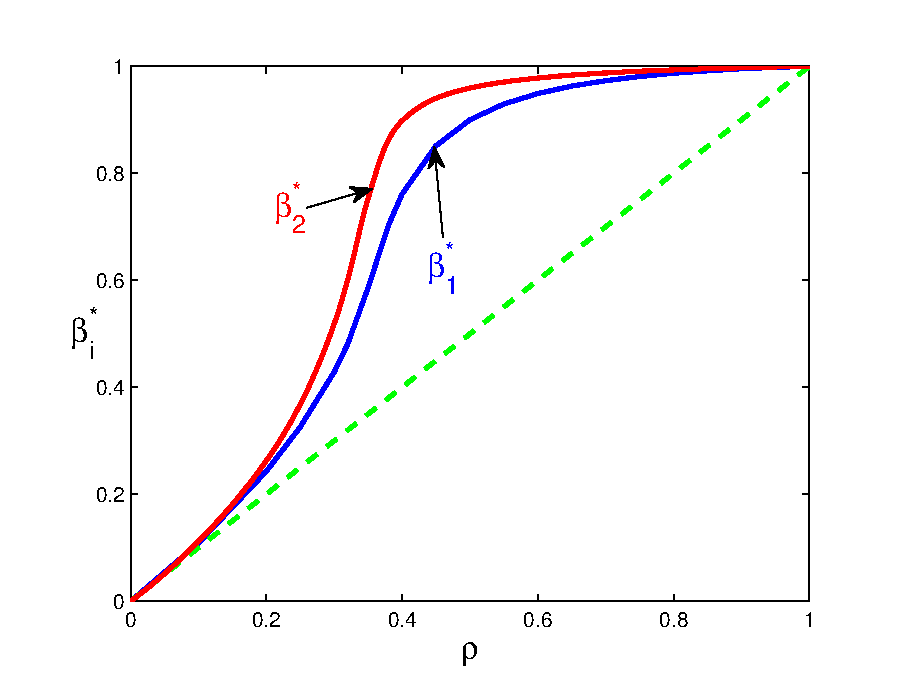
\includegraphics[width=3in]{blerhotrc.eps}}\quad
        \subfigure[]
         {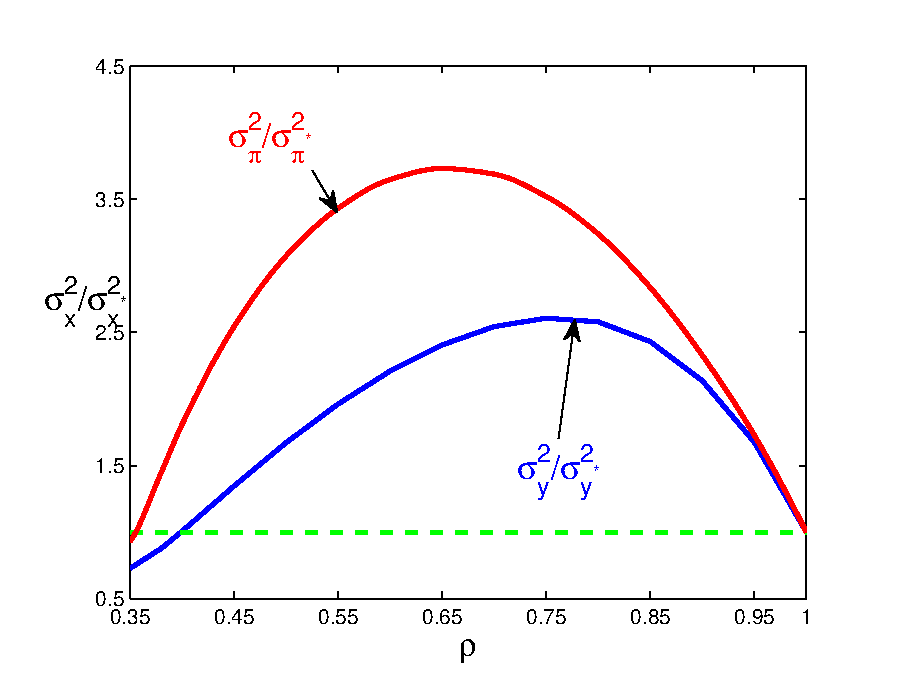
\includegraphics[width=3in]{varrhotrc.eps}}}
   \end{center}
   \caption{ \label{blerhotrc}
   BLE $(\beta^*_1, \beta^*_2)$ as a function of the persistence $\rho$ of the exogenous shocks. (a) $\beta^*_i (i=1,2)$ with respect to $\rho$; (b) the ratio of variances ($\sigma_y^2/\sigma_{y^*}^2$, $\sigma_\pi^2/\sigma_{\pi^*}^2$) of the BLE $(\beta^*_1, \beta^*_2)$ w.r.t. the REE. Parameters are: $\lambda=0.99, \varphi=1, \gamma=0.04, \phi_\pi=1.5,\phi_y=0.5, \frac{\sigma_{\pi}}{\sigma_y}=0.5$. }
\end{figure}



Figure~\ref{blerhotrc} illustrates how these results depend on the persistence $\rho$ of the exogenous shocks. The figure shows the BLE, i.e. the first-order autocorrelations $\beta_1^*$ of output gap and $\beta_2^*$ of inflation, as a function of the parameter $\rho$. This figure clearly shows the {\it persistence amplification} along BLE, with much higher ACF than under RE, for all values of $0< \rho <1$. Especially for $\rho\geq 0.5$ we have $\beta_1^*,\beta_2^* \geq 0.9$, implying that output gap and inflation have significantly higher persistence than the exogenous driving forces. Figure~\ref{blerhotrc} (right plot) also illustrates the {\it volatility amplification} under BLE compared to REE. For output gap the ratio of variances $\sigma_y^2/\sigma_{y^*}^2$ reaches a peak of about $2.5$ for $\rho\approx 0.75$, while for inflation the ratio of variances $\sigma_\pi^2/\sigma_{\pi^*}^2$ reaches its peak of about $3.5$ for $\rho\approx 0.65$. These results suggest that, given the same parameter values, the moments of inflation and output gap implied by BLE and REE are substantially different due to persistence and volatility amplification under BLE. Therefore if the model is estimated on the same dataset under BLE and REE, one might expect important differences in the resulting parameter estimates and the resulting shock propagation mechanism of the model. We explore this implication in the next section by estimating the model under BLE and REE based on U.S. data. 



